
\subsection{Regulering}
Figur~\ref{fig:blokdiagram_regulering} viser et blok diagram for det samlede spændings reguleringsloop. Det viser de overføringsfunktioner samt de to forstærkningsled, der påvirker det samlede system.

\begin{figure}[H]
	\centering
	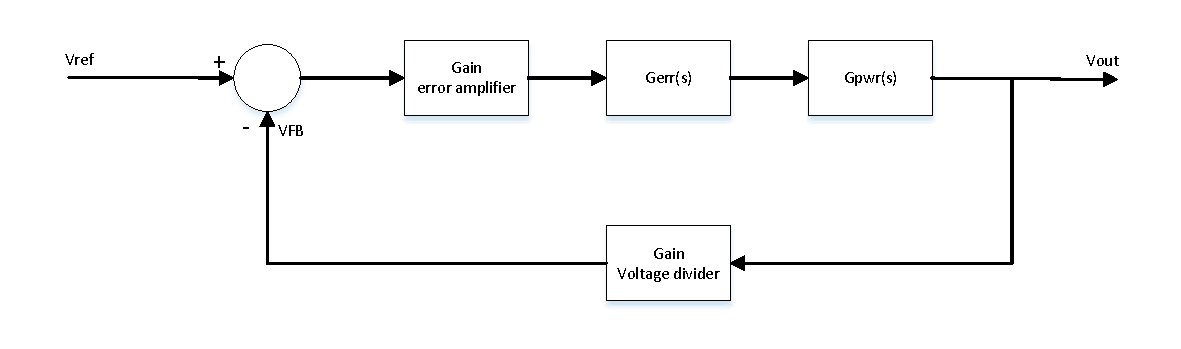
\includegraphics[width=1\linewidth]{../Dokumentation/tex/2iteration/billeder/Regulerings_blokdiagram.pdf}
	\caption{Blok diagram for spænding reguleringsloop}
	\label{fig:blokdiagram_regulering}
\end{figure}

\noindent Der blev først opstillet en overføringsfunktion for power-modulet\cite{UCC1801}. Den indeholder en DC-forstærkning, et nulpunkt fra kondensatorens ESR-modstand og converterens højre halv-plans nulpunkt, samt en pol for belastningen og for switch-frekvensen. 

\begin{equation} \label{H_Power}
G_{pwr}(s) = G_0 \cdot \frac{(1+\frac{s}{2\pi \cdot f_{ESRz}}) \cdot (1-\frac{s}{2\pi \cdot f_{RHPz}})}{1+\frac{s}{2\pi \cdot f_{p1}}} \cdot \frac{1}{1 + \frac{s}{2\pi \cdot f_{p2}} + \frac{s^2}{(2\pi \cdot f_{p2})^2}}
\end{equation}

Der blev genereret et bode plot ud fra overføringsfunktionen, hvilket lagde til grundlag for design af fejlforstærkerens kompensationsnetværk. Det blev besluttet, at det skulle bidrage med en forstærkning på $-5.4\decibel$ med en knækfrekvens på ca. $300\hertz$, for at sikre en stabil converter. Med dette ville der opnås en gain-margin på $24\decibel$, en fasemargin på $74.3^\circ$, og en båndbredde på $810\hertz$.

Dette blev implementeret ved en integrator, der bidrager med en stor DC-forstærkning, og en konstant forstærkning ved frekvenser over knækfrekvensen. 

Overføringsfunktionen for fejlforstærkeren er opstillet ud fra den ønskede knækfrekvens og samlede forstærkning for tilbagekoblingen. Denne forstærkning er et produkt mellem forstærkningen i spændingsdeleren og fejlforstærkeren. 

\begin{equation} \label{H_err}
G_{err}(s) = \left(\frac{f_0 \cdot 2\cdot\pi}{s} + 1\right)  \cdot g_{tot}
\end{equation}

Det er testet ved en integrationstest, der er forklaret i afsnit~\ref{Integrationstest}.

For en mere detaljeret gennemgang af overføringsfunktionernes indhold, og deres bode plots, henvises til dokumentationens afsnit 5.2 og 5.9.4.\fxnote{Indsæt bode plots, beskriv noget med poler og nulpunkter}
\fxnote{Forklar problematikker ved regulering}



